
\section{Museum's role in society}
% TODO: fikse kilder
In the recommendation letter report \emph{“Museums in the society - trust, things and time”} the standing committee of Cultural Affairs present the overall political direction for Norwegian museum policy towards the year 2050. It is established that Norwegian museum institutions take aim at being an expression of both historical and current developments in society. And that museum institutions play an important role in our own time’s understanding of ourselves - both who we have been, who we are, and who we want to be \autocite[p. 7]{melding23}. Modern museum operations is aimed to actively turn to the general public, with the objective to build and share knowledge, increase enlightenment and cultivate cultural capital.

\begin{figure}[h]
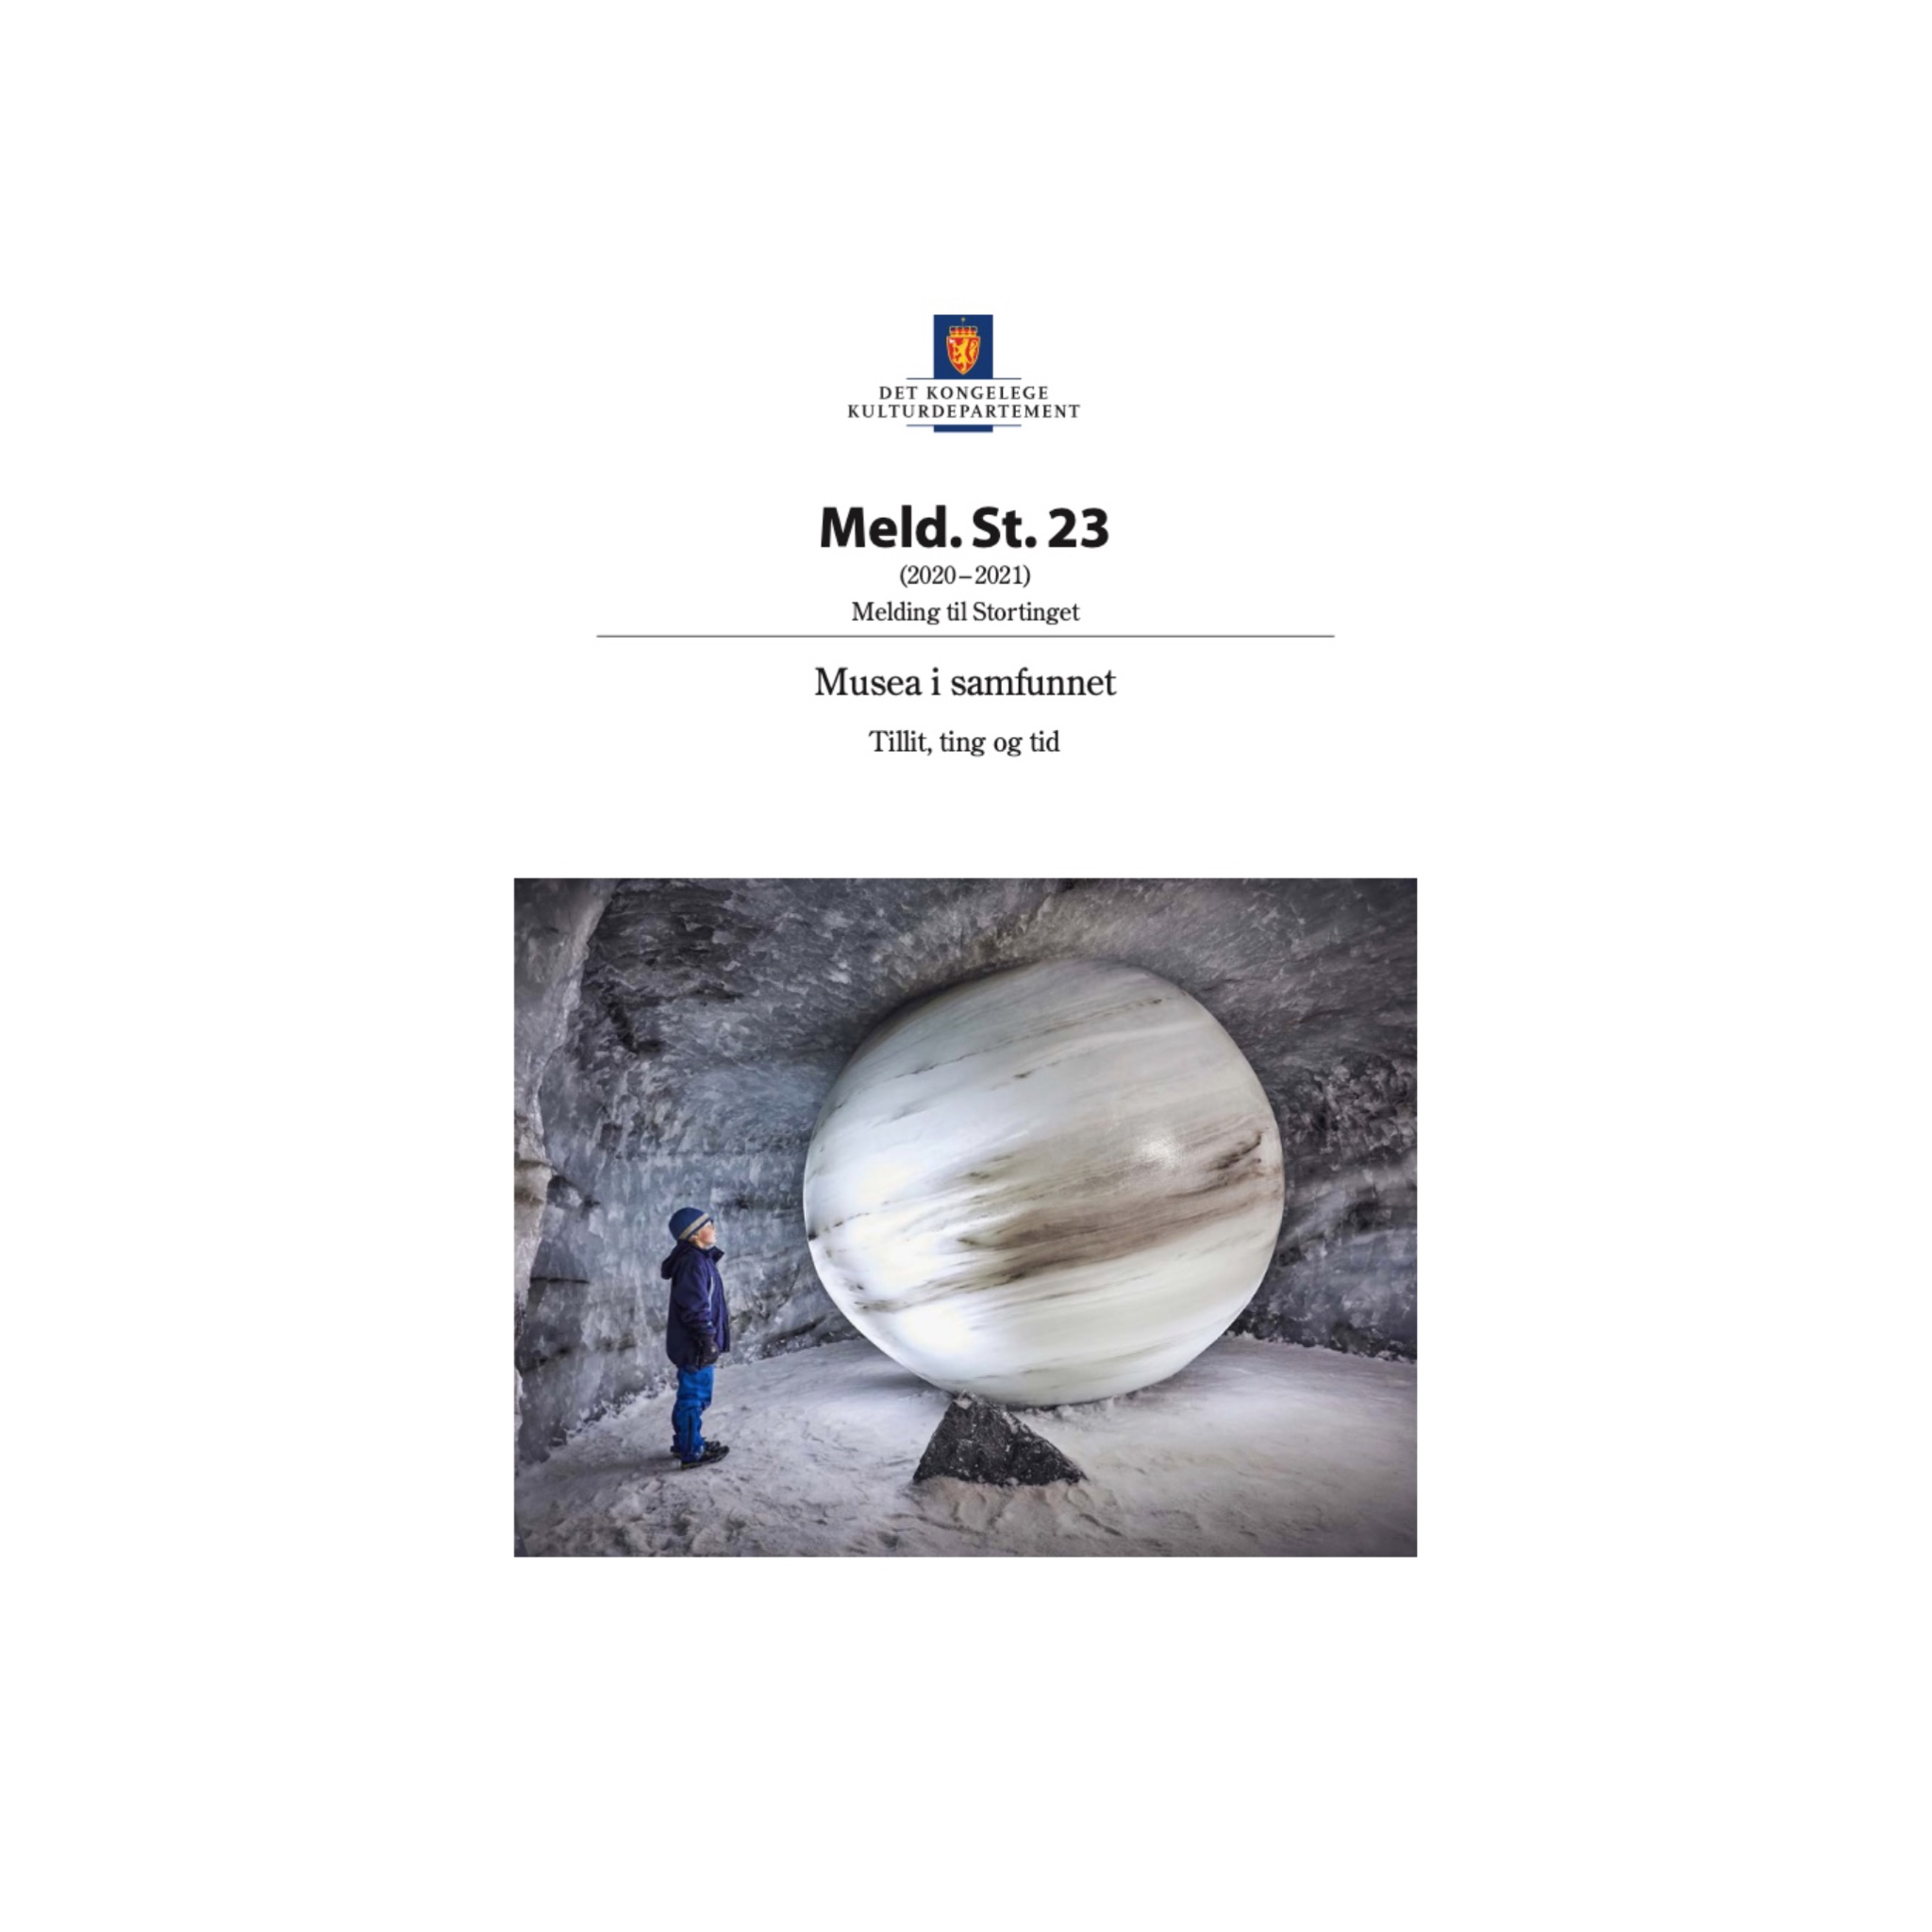
\includegraphics[width=10cm]{pictures/stortingsmelding.jpg}
\centering 
\end{figure}

Where the early museum institutions first and foremost were accessible to a small number of privileged class members, it is now expected that museums purposefully reach out to be open and accessible to all residents and age groups \autocite[p. 14]{melding23}. In Norway, museums are increasingly understood as being both a knowledge- and a social institution, where dissemination and exhibition practice is curated accordingly. At the same time, museums have emerged as an alternative learning arena for school children, first in regards of history teaching, but later in many other subject areas as well. In a society where polarization and public debate is intensifying, arenas that have the public's confidence in being able to nuance and disseminate different perspectives are needed \autocite[p. 7]{melding23}. There is a saying among historians that \emph{"the past teaches us about the present"}. Because history gives us the tools to analyze and explain problems in the past, it positions us to see patterns that might otherwise be invisible in the present – thus providing a crucial perspective for understanding (and solving!) current and future problems \autocite{UW_website}. Being an institution of knowledge, museums have the power to both define and showcase relevant historical events as a perspective to inform present societal issues and debates. 


\section{The new museology}
Museer generelt er i en omstilling fra tradisjonelt "se - ikke rør" til mer interaktivitet i utstillinger. Dette skiftet er en del av en respons på å holde seg relevant som en institusjon, for å appellere til dagens og fremtidens museumsbesøkende. Her spiller ny bruk av teknologi inn, samt mer interaktivitet i utstillingene og høyere "krav" til at museet skal være engasjerende og kunne tilbringe noe som er gøy. Museer prøver å bryte opp i forestillingen mange har om at det er kjedelig å gå på museum. Samfunnsinstitusjoner som biblioteker går også gjennom samme type transition. "hva er det moderne museet?" - "hva er det moderne biblioteke"?. Museet er i tillegg en samfunnsinstitusjon med en unik posisjon til å være en arena for læring, hvor man kan stole på at informasjonen er korrekt/ til å stole på. 

En del av en større samfunnsmessig omveltning/ transition mot noe "mer moderne". Rebirth! :P

Today’s teenagers and young adults are the future generation of museum-visitors, and contemporary discourses like the climate crisis demands an active discussion across all age-groups. % Denne målgruppen skiller seg ikke bare fra andre på grunn av alderen, men særlig på grunn av deres forhold til og bruk av teknologi. Digitale flater og plattformer brukes i stor grad for å orientere seg om hva som skjer i verden, og i sosiale kretser. De er mer "tech savvy", og man må kjempe hardere for å fange og holde på oppmerksomheten deres. Målgruppen er spennende å jobbe med fordi 

\section{Exhibition practise}

\subsection{Artefact vs artwork}
The ethnographic museum conserves and exhibits artefacts, while the art museum, works of art. It seems obvious what differs the artefact vs the artwork; yet in this section we will learn how the objects they refer to differ regarding what they represent. Both artefacts and artworks is charged with cultural meaning. It tells us about a larger cultural situation, e.g. aesthetic conceptions or world views, conceptions of representations or the social relevance of art. These meanings is only yielded if we are able to “read” it, or is put in some context that illuminates the cultural meaning \autocite[p. 206]{Thi_book}.

The term artefact suggests a man made object charged with cultural meaning which can, if studied carefully, offer us information on the society in which it has been created \autocite[p. 205]{Thi_book}. The difference between the artefact according to the above definition and the common idea of art is that the former takes for granted what the other represses: the possibility of cultural difference. Instead, artworks are viewed as standing for an aesthetic, and is therefore considered metaphors, transferring their specific aesthetic to the one current sufficient to make the work “readable” as art, regardless of what it could tell us about the culture it comes from \autocite[p. 206]{Thi_book}. While the ethnic artefact, in contrast, is first and foremost considered to be a representative of the larger context of the culture it comes from \autocite[p. 206]{Thi_book}. Hence, it is not a metaphor but synecdoche. Synecdoche is the figure of rhetoric where an element, a small part, stands for the whole simply by virtue of its being a part of that whole \autocite[p. 206]{Thi_book}. Thus the artefact is only readable as culture, no matter what aesthetic qualities it may also have.

% need more

\subsection{The curator}
The curator are, above all, the institutionally recognised experts of the artworld establishment, whether they operate inside an institution or independently. More than art critics or gallery dealers, they establish the meaning and status of contemporary art through its acquisition, exhibition, and interpretation \autocite[p. 22]{Thi_book}. To a greater extent than other artworld professionals, curators additionally depend on an established infrastructure to support their efforts. This infrastructure includes institutionalised networks, such as those provided by museums, galleries, or alternative spaces; financial sponsors, whether public, private or corporate, and teams of technical or professional experts. Curators are the sanctioned intermediaries of these institutional and professional networks on the one hand, and; artists and audiences on the other. Curatorial function is, this, inherently restricted by the interests of the larger or more powerful groups and constituencies \autocite[p. 22]{Thi_book}.

By selecting, framing and interpreting peripheral art in exhibitions and exhibition catalogues, for instance, art curators can claim to be shaping a more democratic space where specific cultural groups can recognise themselves \autocite[p. 23]{Thi_book}. As the debates of recent years have shown, “identity” is not an “essence” that can be translated into a particular set of conceptual or visual traits. It is, rather a negotiated construct that results from the multiple positions of the subject vis-a-vis the social, cultural and political conditions which contains it. How then, can exhibitions or collections attempt to represent the social, cultural and political complexities of groups without reducing their subjects to essentialist stereotypes? \autocite[p. 23]{Thi_book}.

This situation places the cultural broker at the very core of a contradiction: on one hand, she can be credited for helping to tear down artworld hierarchies, seemingly democratizing the space for cultural action; on the other hand, in a market scenario where “identity” can only be a reductive construct, the framing and packaging of images of the collective self can only result in a highly delusionary enterprise \autocite[p. 23-24]{Thi_book}. The tensions of this contradiction confront art curators with a dilemma. where should they position themselves vis-a-vis the identities of the groups they claim to respect? \autocite[p. 24]{Thi_book}.


\subsection{Discursivity and cultural moralism}
Discursivity, most notably rhetoric imbricated with narrative is in effect a crucial aspect of the museum institution \autocite[p. 205]{Thi_book}, it is the core of the idea of exhibition.

The museum is an attractive object of study, because it requires interdisciplinary analysis, it has the debate on aesthetics at its core, and that it is essentially a social institution (Thi, p. 202). Mieke Bal account for and describe the issue of cultural imperialism in museums, exemplifying case studies related to natural history types of museums that conserves and display ethnic objects and artefacts representing cultures and cultural properties from the past. The ethnographic museum is clearly the most obviously politically charged institution, and it poses the immediate problem of cultural property and collective ownership (Thi, p. 202). It raises the question if former colonists are entitled to hold onto objects taken by their ancestors from former colonies, or should they give these back to the country of origin the ancestors of whose inhabitants were their original owners?

I think this (as a sort of ethical) perspective is necessary to have in this context, because the intention of making a meaningful interactive experience is to strengthen the message conveyed by the museum. Both the designer and especially the museum need to be aware of and able to answer moral and ethical questions in terms of what the message they convey actually conveys. And that the act of strengthening that impression in a greater way sends people out of the museum with reflections and thoughts that leads to social action (climate action, consciousness). 




\subsection{Installations}
Data, as in information, holds a lot of the evidence and arguments as to why we as a society and the visitor as an individual need to transition into a more sustainable way of living. And is therefore also relevant to analyse and look at in the same way we would do an artefact or installation on display in regards to Klimahuset.



\section{Types of visitors}
In this section I want to write a bit about the different types of visitors that exist in the museum. And then adding in "new" types of visitors in a hybrid space (interacting visitors).

Thinking:
- The observator
- The interactor
- the young one
- the old one
- ..... ??

\par Need to find some literature on thissss..